\documentclass[10pt]{article}
\usepackage[T1]{fontenc}
\usepackage[utf8]{inputenc}
\usepackage{lmodern}
\usepackage[margin=0.7in]{geometry}
\usepackage{amsmath,amssymb}
\usepackage{microtype}
\usepackage{multicol}
\usepackage{enumitem}
\usepackage{graphicx}
\usepackage[font=small,labelfont=bf,skip=3pt]{caption}
\usepackage[dvipsnames]{xcolor}
\usepackage[backend=bibtex,style=authoryear,natbib=true,maxcitenames=2,maxbibnames=4,minbibnames=3,uniquelist=false,uniquename=false,giveninits=true,doi=false,isbn=false,url=false,eprint=false]{biblatex}
\addbibresource{refs.bib}
\usepackage[colorlinks=true,linkcolor=MidnightBlue,citecolor=MidnightBlue,urlcolor=MidnightBlue]{hyperref}
\usepackage[capitalise,nameinlink]{cleveref}
\setlength{\parskip}{3pt}
\setlength{\parindent}{0pt}
\setlist{nosep,leftmargin=*}
\setlength{\textfloatsep}{8pt}
\makeatletter
\renewcommand\paragraph{\@startsection{paragraph}{4}{\z@}{1.0ex \@plus .3ex \@minus .2ex}{-1em}{\normalfont\normalsize\bfseries}}
\renewcommand\maketitle{\begin{center}{\large\bfseries\@title\par}\vspace{3pt}\@author\quad\textperiodcentered\quad\@date\end{center}}
\makeatother
\newcommand{\extra}{\textsuperscript{\dag}}

\title{Together First, Apart Later? When Optimizers Start to Learn Different Functions\\[1pt]
\normalfont Initial checkpoint, MIT 6.7910, Fall 2026}
\author{Juntang Wang and V\'ictor Conchello}
\date{October 30, 2026}

\begin{document}
\maketitle
\vspace{-0.8em}

\paragraph{Question.} From the same initialization and the same sequence of mini-batches, do SGD with momentum,
AdamW and Muon first follow the same path in function space and only later separate? If so, where is the split,
what coincides with it (an edge-of-stability event \citep{cohen2021eos,cohen2022adaptive}, the end of warmup, a
loss level), and is the final function already decided there?

\paragraph{What we have done.} We trained nanoGPT \citep{karpathy2022nanogpt} on character-level
Shakespeare (10.8M parameters) and TinyStories-10M and -30M (14M and 30M parameters) with SGD, AdamW and Muon
\citep{jordan2024muon}, at learning rates from a sweep, from a shared initialization and with five data orders
per optimizer. Along training we logged the next-token predictions on fixed held-out contexts, and the top
Hessian eigenvalue and AdamW's preconditioned one by Lanczos. We swapped optimizers at nine fork steps with warm
optimizer states, measured linear mode connectivity, and replicated the CIFAR-10 break-even analysis
\citep{jastrzebski2020breakeven}. In total 392 runs, about 103 GPU-hours. Items added beyond the plan are
marked \extra.

\paragraph{Method.} The distance between two runs is the mean Jensen--Shannon divergence of their next-token
predictions. We compare runs at equal \emph{training loss}, so that one optimizer being faster is not counted
as a difference, and divide by a noise floor: the distance between two runs of the same optimizer that differ
only in data order. A split is a stretch of loss levels where this ratio exceeds 1.5; it is persistent\extra\
if it lasts to the end of training, with a bootstrap over data orders for its location.

\begin{figure}[h]
\centering
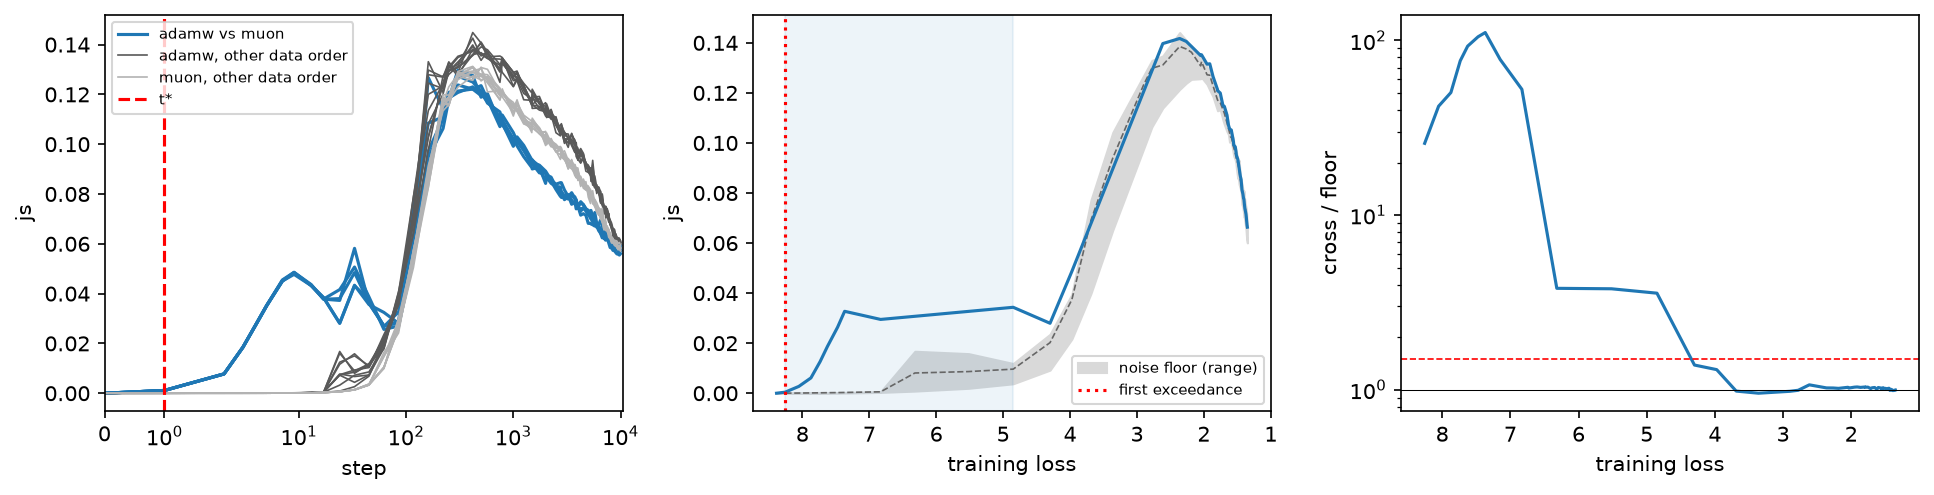
\includegraphics[width=0.92\linewidth]{figures/ts10m/divergence_adamw_muon.png}
\caption{AdamW against Muon on TinyStories-10M, five data orders. Left: distance at equal steps (blue) and the
data-order floor (grey). Middle: at equal training loss, with the floor's range; shaded, the episode above
the floor. Right: their ratio, with the split threshold 1.5 (red).}
\label{fig:div}
\end{figure}

\paragraph{Result 1: apart first, together later (\cref{fig:div,fig:overview}).} At equal steps the optimizers
differ from the first steps, mostly because they progress at different speeds. At equal loss, in all three
settings and for every pair, the distance is 30--200 times the floor at high loss and falls back to about the
floor around the stage at which the models have learned the bigram statistics of the data. On TinyStories it
stays there: at the end of TinyStories-30M, replacing AdamW by Muon changes the predictions no more than
changing the data order. Of the nine pairs only Muon--SGD on Shakespeare, where SGD barely trains, has a
persistent split, and it is lost with another metric or a stricter threshold. The answer to the title is
therefore the reverse of the hypothesis: the optimizers' functions differ early and meet later.

\begin{figure}[h]
\centering
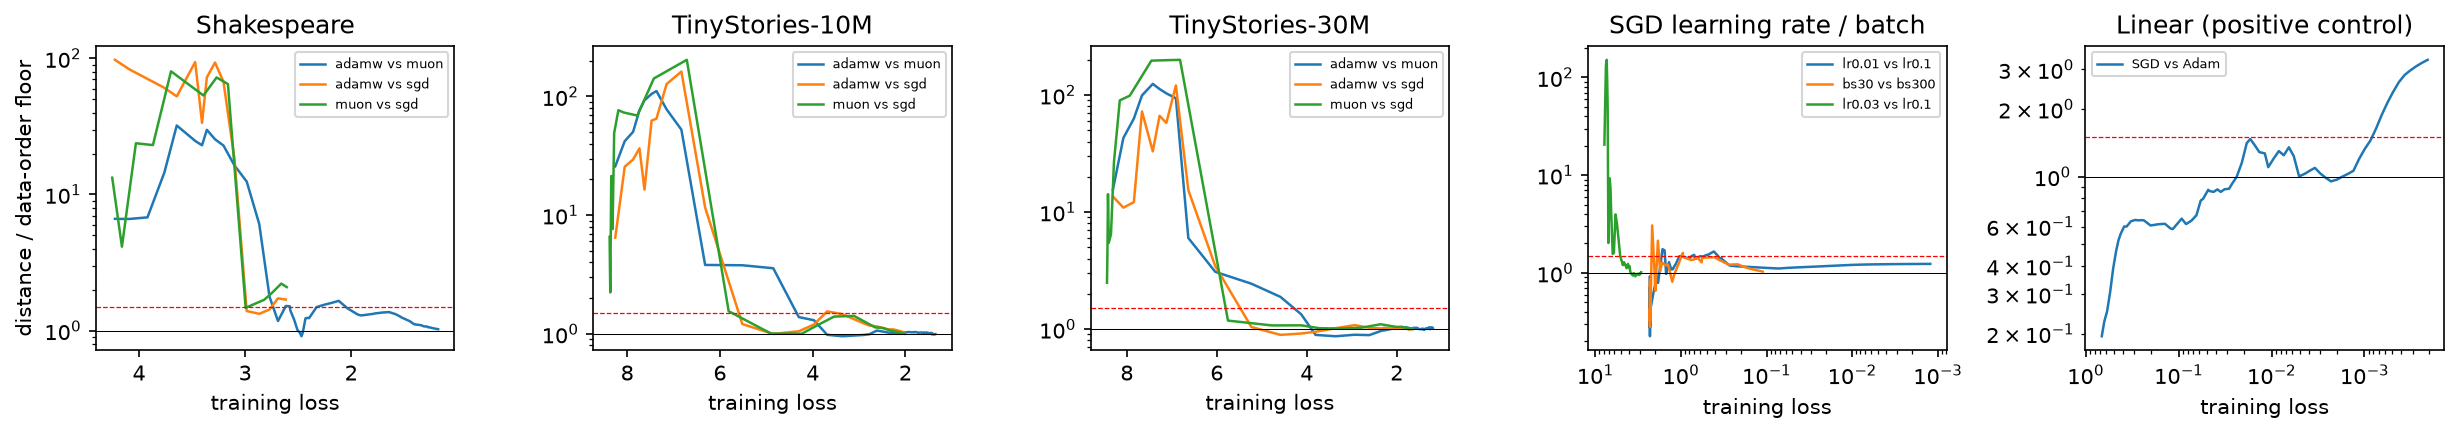
\includegraphics[width=0.85\linewidth,trim=0 198 0 0,clip]{figures/overview.png}
\caption{Loss-matched distance between optimizers over the data-order floor (training progresses to the right);
red dashed, the threshold 1.5. Red, left\extra: AdamW--Muon trained into memorization (8000 steps).}
\label{fig:overview}
\end{figure}

\paragraph{Result 2: no edge-of-stability event at the split.} On TinyStories AdamW's preconditioned
sharpness sits at its threshold $(2+2\beta_1)/((1-\beta_1)\eta)$ for much of training, whether or not the
optimizers differ, and SGD reaches $(2+2\mu)/\eta$ only early in training. The early episodes end within warmup
(steps 9--85), the same way for AdamW--Muon, where SGD is not involved. A stage of learning describes the
re-convergence better than a stability event.

\paragraph{Result 3: the last optimizer decides the function (\cref{fig:swap}).} When we switch optimizer at
step $t$, the fork ends within the floor of the new optimizer whenever that optimizer is fast enough to get
there in the remaining steps: forks from SGD to AdamW or Muon land on the new optimizer even after 4000 of
10{,}000 steps, while forks into the slower SGD end closer to their parent from step 1500 on (step 5000 on
TinyStories-30M). The endpoint is thus not decided early. Weight space keeps a mark that function space does
not: after a change of optimizer, a fork needs a later fork step to stay linearly connected to its parent
\citep{frankle2020lmc} than after a change of data order.

\begin{figure}[h]
\centering
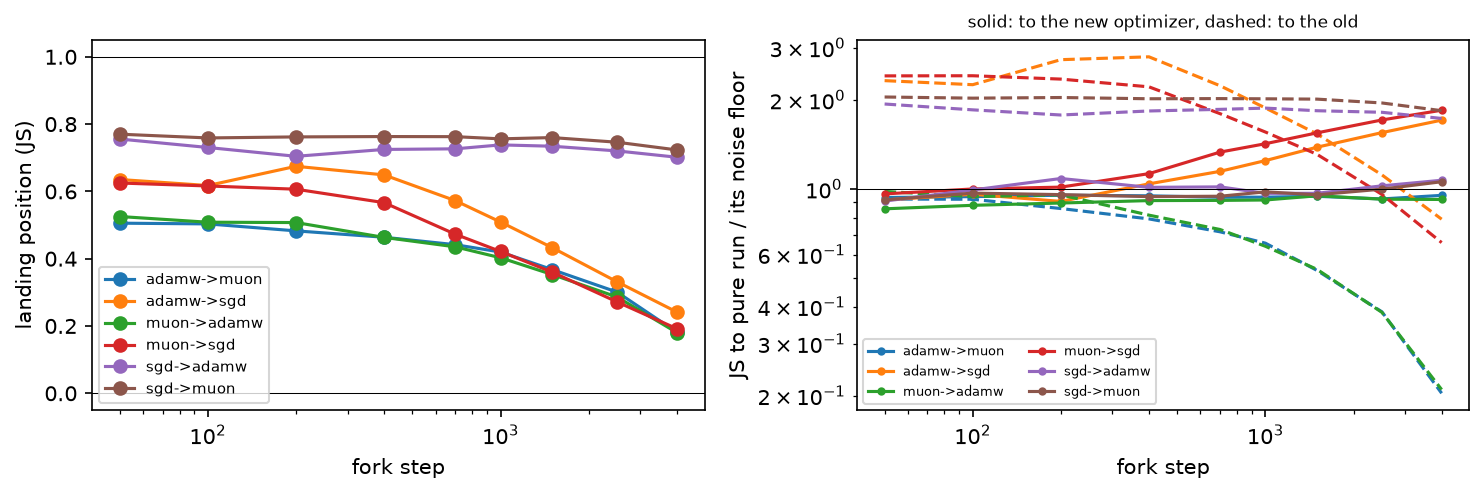
\includegraphics[width=0.8\linewidth]{figures/ts10m/swap.png}
\caption{Swaps on TinyStories-10M. Left: where the fork ends between pure $A$ (0) and pure $B$ (1). Right\extra:
its distance to pure $B$ (solid) and to pure $A$ (dashed) in units of their floors; below 1 means
indistinguishable from that optimizer.}
\label{fig:swap}
\end{figure}

\paragraph{Result 4 (moonshot, first look).} The top Hessian eigenvector lies in different blocks for each
optimizer: Muon's in the value--output matrices on TinyStories and in the embeddings on Shakespeare, AdamW's in
the head and later the LayerNorm gains, SGD's spread over MLP, value--output and head. In all three, 70--85\% of
the eigenvalue comes from curvature \emph{between} blocks rather than within one. Of the part of the direction in the
transformer blocks, most lies in the first two (one run per optimizer, TinyStories-30M). Its changes of block come long after the optimizers have
re-met, so they do not mark a split.

\paragraph{Pipeline check and controls.} On CIFAR-10 the break-even effects replicate: the sharpness levels off
at or below $2/\eta$ and lower for larger rates, and the gradient covariance is better conditioned; but at equal
loss two learning rates differ by at most about twice the floor. Controls\extra: a second initialization
reproduces the results, and on a linear model on separable data, where gradient descent and Adam have different
max-margin limits \citep{soudry2018separable,zhang2024adam}, the same test does find a persistent split.

\paragraph{Next (Nov--Dec).} (i) Moonshot: which layers carry the sharp direction \emph{at} the edge of
stability, restricted to the steps at the threshold and averaged over the five data orders; whether it moves to
the new optimizer's layers after a swap; and a causal test lowering the learning rate of only those layers.
(ii) Robustness of the split rule to the metric and the threshold. (iii) Presentation (Dec 1--4), paper, code
and Colab notebook (Dec 5--11). Code: \url{https://github.com/qqgjyx/MIT-6.7910}.

{\scriptsize\setlength{\bibitemsep}{0pt}\begin{multicols}{2}\printbibliography[heading=none]\end{multicols}}

\end{document}
